\section{Supervisión de servidor de servidor de acceso remoto (SSH)}
\subsection{Instalación}
Para el desarrollo de esta práctica se optó por implementar el protocolo SSH \textit{Secure Shell}. La instalación de este servidor de acceso remoto es muy simple. Basta con ejecutar el comando:\\
\texttt{apt-get install openssh-server}\\

En caso de que el servicio no sea iniciado automáticamente después de la instalación se ejecuta el comando:\\
\texttt{service sshd start}\\
\subsection{Sensor SSH}
Para la implementación del sensor se monitorizaron 4 aspectos: el número total de conexiones, dirección IP origen, dirección IP destino y usuario al que se encuentra conectada la sesión.
Para obtener estos datos se ejecuta la función \textbf{sensor\_ssh()} del programa \textbf{cliente.py}. En la figura \ref{image:sensorsshcodigo} se puede observar a detalle el código.

\FloatBarrier
\begin{figure}[htbp!]
		\centering
			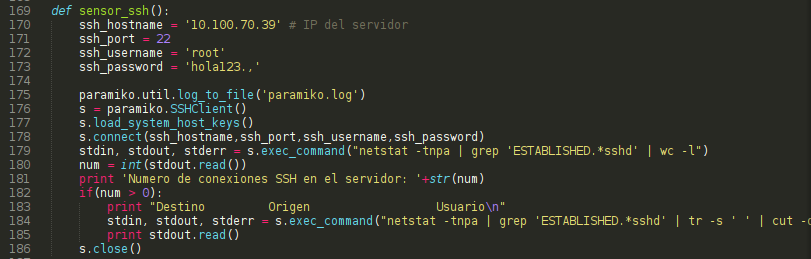
\includegraphics[width=.65 \textwidth]{images/sensorsshcodigo}
		\caption{Código del sensor SSH.}
		\label{image:sensorsshcodigo}
\end{figure}
\FloatBarrier

En esta función podemos ver que se realiza una conexión SSH al servidor para ejecutar el comando \texttt{netstat -tnpa | grep `ESTABLISHED.*sshd' | wc -l } para obtener el total de conexiones SSH establecidas. Si el número de conexiones es mayor a cero se ejecuta el comando \texttt{netstat -tnpa | grep `ESTABLISHED.*sshd' | tr -s ` ' | cut -d` ' -f4,5,8} con lo cual se obtiene la información requerida por cada conexión establecida.

\subsubsection{Funcionamiento}
La ejecución de este sensor se puede observar en la figura \ref{image:sensorsshfunc}

\FloatBarrier
\begin{figure}[htbp!]
		\centering
			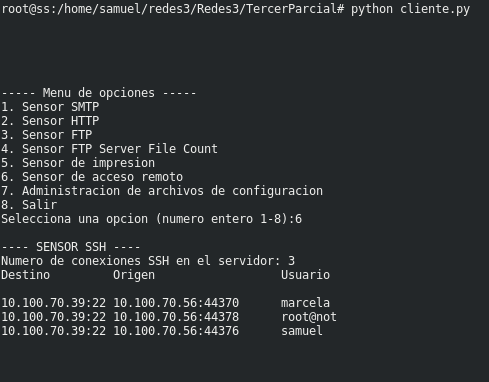
\includegraphics[width=.55 \textwidth]{images/sensorsshfunc}
		\caption{Funcionamiento del sensor SSH.}
		\label{image:sensorsshfunc}
\end{figure}
\FloatBarrier

Este resultado se obtiene al tener iniciadas dos sesiones de SSH como se muestra en la figura \ref{image:sshconn}.

\FloatBarrier
\begin{figure}[htbp!]
		\centering
			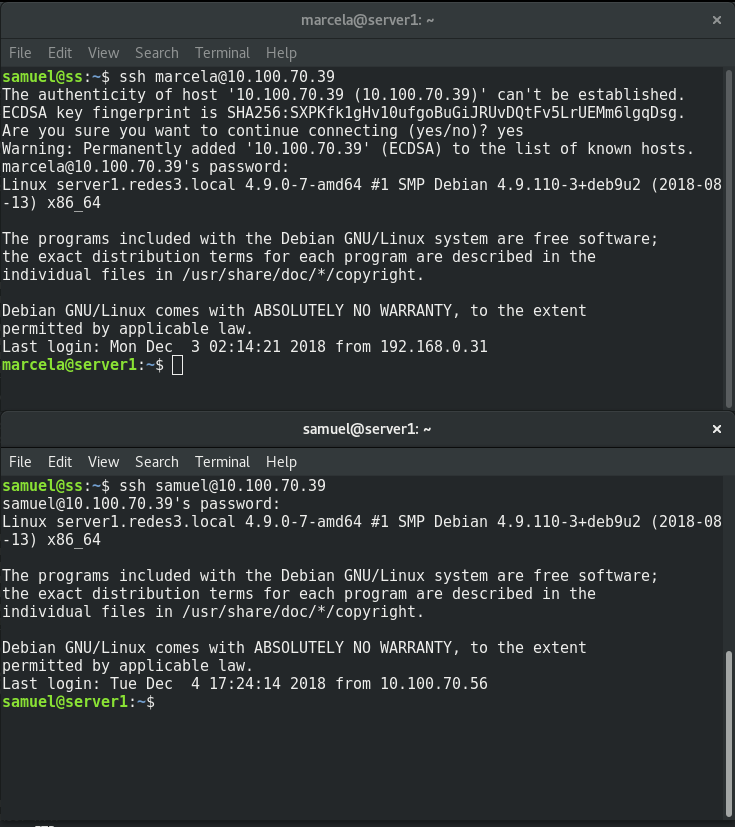
\includegraphics[width=.55 \textwidth]{images/sshconn}
		\caption{Conexiones SSH.}
		\label{image:sshconn}
\end{figure}
\FloatBarrier

Es importante recalcar que el sensor reporta 3 sesiones ya que también cuenta la sesión que utiliza el mismo sensor para obtener los datos.